\capitulo{5}{Aspectos relevantes del desarrollo del proyecto}\label{cap:relevantes}

En este capítulo se explicarán las partes más importantes del desarrollo del proyecto.

\section{Desarrollo de la aplicación web}

Para realizar la primera fase del desarrollo, la recogida de los datos, se ha desarrollado una aplicación web que facilitase las tareas de telerrehabilitación conectando al personal especializado con los pacientes con enfermedad del \textit{Parkinson}. Esta recogida se hizo incorporando dentro de sus funciones la grabación a los mismos durante la realización de los ejercicios para ser estudiados en tiempo real. 

Dentro del funcionamiento natural del flujo, se incorpora una función de anonimización del rostro para mantener la intimidad de los pacientes en los estudios posteriores sobre el material grabado, además no se guardan datos identificativos de ningún paciente.

Esta aplicación se ha compuesto de dos partes. Una ha consistido en el diseño y consecuente implementación de una interfaz hombre-máquina fácil de usar y accesible mediante un mando sencillo\footnote{Concretamente un mando de la consola SNES adaptado para ser usado mediante USB.}. Esta se compone de una serie de botones de colores, directamente relacionados con los del mando~(figura~\ref{fig:help}), que permiten iniciar una comunicación mediante videoconferencia con el personal terapéutico y finalizar la reunión. Durante el proceso de la llamada, el vídeo del paciente es capturado y enviado al servidor para su procesado en tiempo real.

\begin{figure}
	\centering
	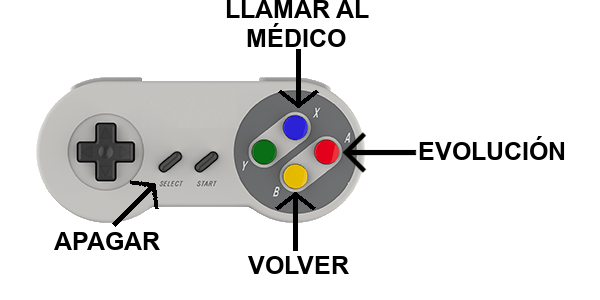
\includegraphics[width=0.7\textwidth]{img/ayuda.png}
	\caption{Funcionalidades del mando de SNES para el control de la aplicación web por parte del paciente.}
	\label{fig:help}
\end{figure}


En la \autoref{fig:clientedesplegado} se puede observar el equipo destinado para el uso por parte del paciente ya instalado y listo para usar.

\begin{figure}
	\centering
	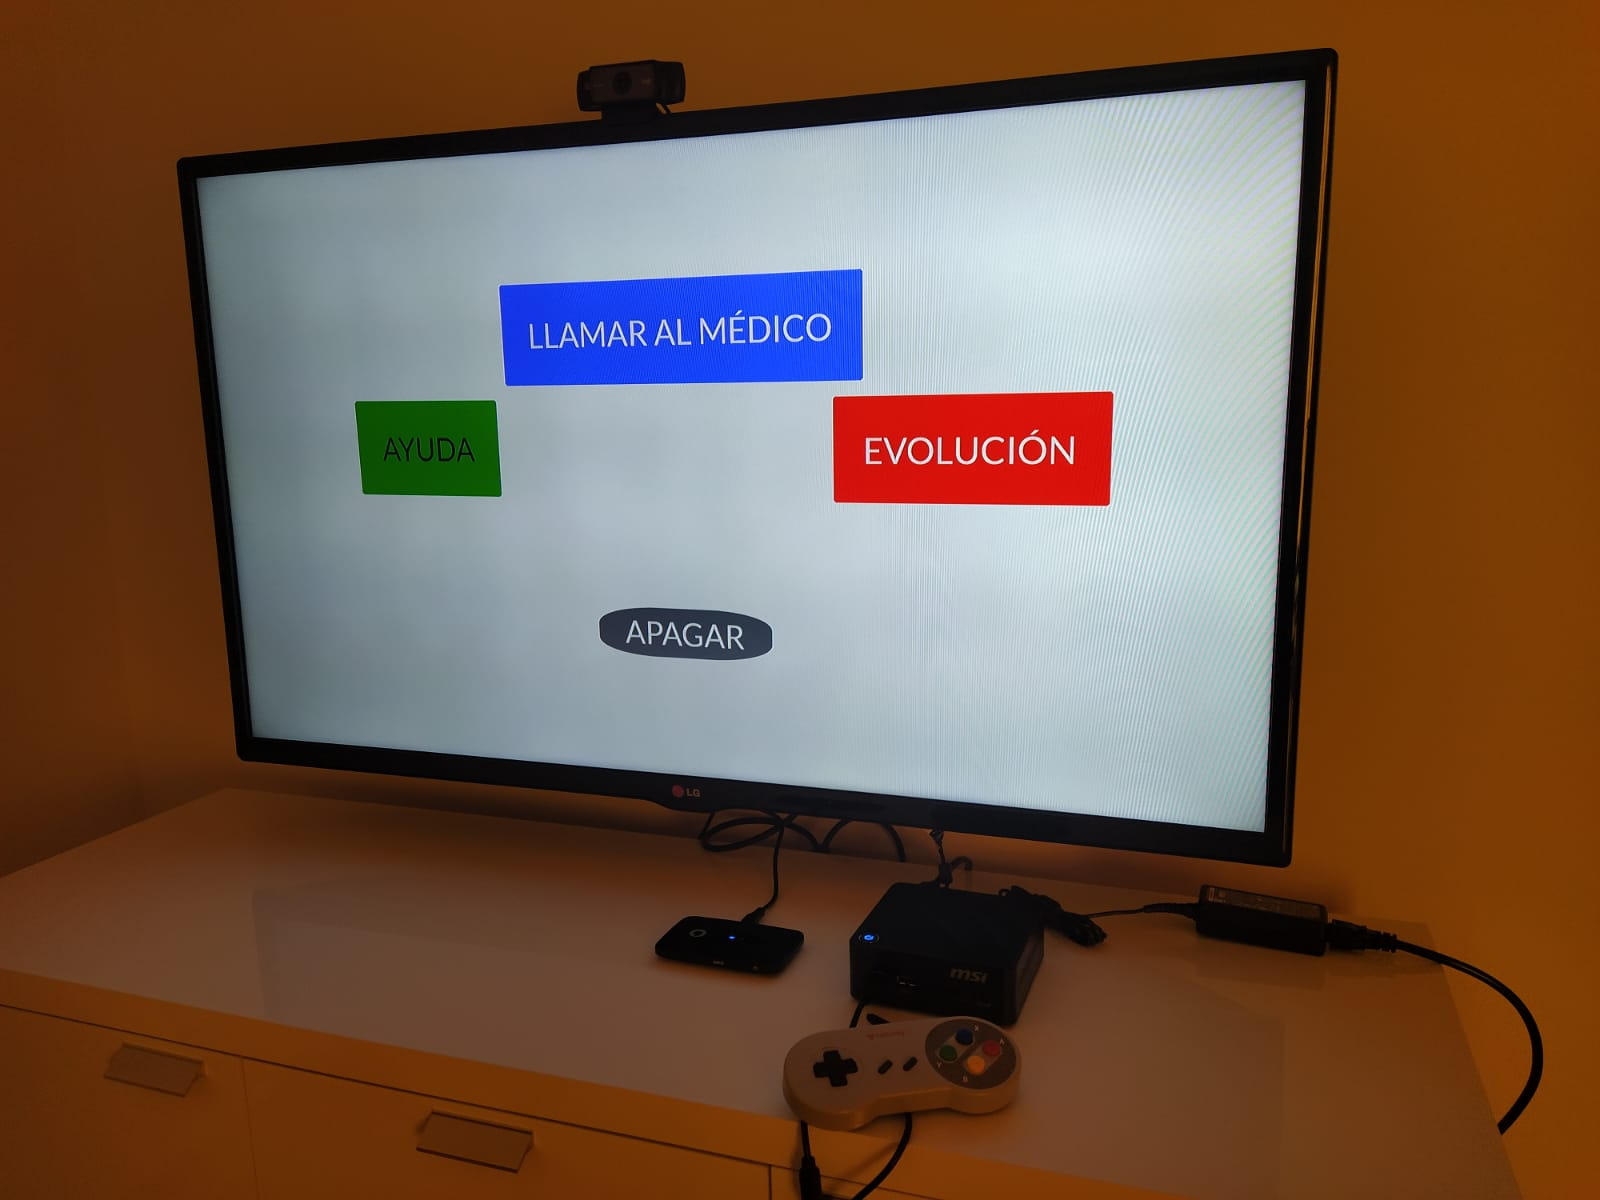
\includegraphics[width=0.8\textwidth]{img/desplieguefisico2.jpeg}
	\caption{Cliente para el paciente sobre el soporte instalado en el domicilio del paciente.}
	\label{fig:clientedesplegado}
\end{figure}

La segunda parte consiste en la interfaz del terapeuta encargado de dirigir las sesiones de rehabilitación del paciente ofreciendo una interfaz sencilla que permite conectarse a las videoconferencias de los diferentes pacientes y dirigir las sesiones de terapia, además de gestionar la evolución del paciente~(figura~\ref{fig:menu_respon}).

\begin{figure}
	\centering
	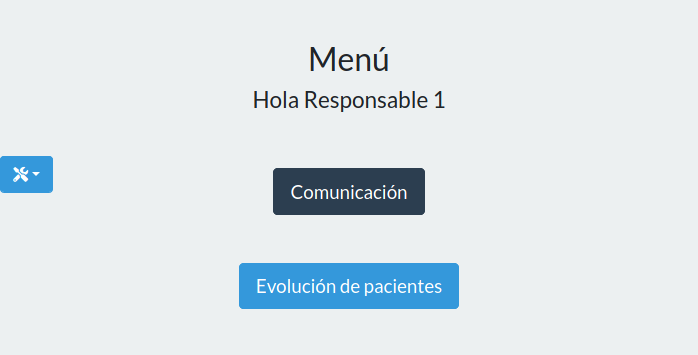
\includegraphics[width=0.8\textwidth]{img/menu_responsable.png}
	\caption{Menú del terapeuta}
	\label{fig:menu_respon}
\end{figure}

Las características del equipo donde está desplegada la aplicación del paciente es:
\begin{itemize}
	\item MSI -- Cubi N 8GL-001BEU N4000 1.10GHz.
	\item WB Green M.2 120 GB SATA 3.
	\item 4 GB DDR4 2400 MHz.
	\item Lubuntu x86\_64 18.04.
	\item WebCam Logitech HD Pro C920.
\end{itemize}

\subsection{Herramientas utilizadas}\label{sec:recogidadatos}

Este servicio se divide en tres partes: el \textit{backend}, el \textit{frontend} y el servicio de \textit{streaming} de vídeo.

\subsubsection{\textit{Backend}}

El \textit{backend} es el conjunto de servicios en el lado del servidor de un servicio web. Para construirlo se han utilizado dos librerías de \textit{Python}.

\textbf{Jinja~\cite{tool:jinja}}: gestor de plantillas de código abierto (BSD), se utiliza para la creación de la interfaz web mediante la creación de páginas dinámicas en HTML.

\textbf{Flask~\cite{tool:flask}}: \textit{microframwork} de código abierto (BSD) que ofrece una capa de abstracción muy alta de un servicio web, se utiliza para la creación de la lógica de negocio mediante la gestión de las rutas.

\subsubsection{\textit{FrontEnd}}

El \textit{frontend} es la parte del servicio web que muestra la información al cliente y permite la interacción con el mismo. Se han usado dos \textit{frameworks} para \texttt{HTML5}.

\textbf{Bootstrap~\cite{wiki:boostrap}}: \textit{Framework} de \textit{CSS} de código abierto (MIT) creado por \textit{Twitter} para la creación de aplicaciones web redimensionables. Todos los estilos de la web se apoyan en este \textit{framework}.

\textbf{jQuery~\cite{wiki:jquery}}: \textit{Framework} de \textit{JavaScript} de código abierto (MIT) que simplifica el acceso al \textit{HTML DOM} de la página. La gestión de los eventos de la web se gestionan mediante este \textit{framework}.

\section{Implementación del flujo}

Los componentes del flujo ETL implementado (\autoref{fig:flujoetlreal}) se realizaron mediante tres \textit{scripts} de \textit{Python} según las tres etapas del flujo. Primero un emisor \textit{UDP} de vídeos que simula la entrada de los vídeos de los pacientes. El segundo \textit{script} es el ingestor en \textit{Kafka} de los fotogramas del vídeo recibido. Por último, el tercero es el procesador de los diferentes \textit{frames} mediante \textit{Spark} y \textit{OpenCV}.

El \textit{script} emisor consiste en un cliente \textit{UDP} que itera sobre los fotogramas del vídeo y los comprime mediante la abstracción de \textit{DEFLATE} \textit{zlib}~\cite{tool:zlib} sobre la imagen serializada bajo el estándar \textit{JPEG/Exif}~\cite{pennebaker1992jpeg} con una calidad del 95\%. Esta compresión del fotograma permite que la velocidad de encolado se minimice. Además este \textit{script} simula la tasa de refresco de un vídeo real emitiendo a quince fotogramas por segundo, las frecuencia de los vídeos reales que se capturarán con los pacientes.

El segundo \textit{script}, el ingestor, se divide en dos partes, una encargada de la escucha de los paquetes \textit{UDP} que se reciban por parte del emisor, y otra destinada al encolado de los fotogramas en un productor de \textit{Kafka}. El servidor \textit{UDP} se implementa  mediante un \textit{socket} de flujo (\texttt{SOCK\_STREAM}) de tal manera que no es necesario conocer el tamaño del paquete con anterioridad dando así más flexibilidad al flujo completo. Respecto a la emisión al productor de \textit{Kafka} el fotograma comprimido se envía junto a una clave que indica el número dentro de la secuencia del vídeo.

El último componente es el procesador de las imágenes. Consiste en un flujo de \textit{Spark Streaming} que se conecta a un \textit{topic} de \textit{Kafka}. Este es el punto más extensible del flujo ya que la mayor dificultad está en la conexión previa que se ha de hacer. La configuración básica está en procesar cada \textit{frame} por separado mediante el sistema de \textit{microbatching} que utiliza \textit{Spark}, pero se puede configurar para hacer ventanas deslizantes con los que procesar varios fotogramas. Se incorpora un proceso sobre las imágenes para la anonimización mediante la detección del rostro usando el modelo de \textit{Caffe}~\cite{jia2014caffe} y aplicándole un filtro gaussiano o una reducción de resolución (para más información ver la sección~\ref{sec:manualpro}) Adicionalmente se ha incorporado un algoritmo de corrección del contraste y del brillo.

Debido al funcionamiento de \textit{Spark Streaming} se pueden acoplar más funciones. Aunque cuantas más sean, más se realentizará el proceso y con ello se puede perder el factor de <<tiempo real>> en el análisis del flujo. El objetivo con esto es que el trabajo del compañero José Miguel Ramírez Sanz se pueda incluir como el último paso en el procesado del vídeo.

\subsection{Limitaciones}

Debido a la naturaleza de las herramientas utilizadas existen algunas limitaciones importantes a mencionar.

La principal limitación está en el tiempo sobre las acciones alrededor de \textit{Apache Kafka}, ya que existen tres momentos temporales que poseen máximos técnicos. El primero es el tiempo de encolado, si un paquete tarda mucho en ser insertado al \textit{topic} correspondiente este es rechazado, la velocidad de este proceso está fuertemente ligado al tamaño del paquete emitido. El segundo tiempo es el tiempo de vida del paquete dentro de la cola y si un paquete está más tiempo en la cola que este tiempo es automáticamente rechazado. Por último está el tiempo de desencolado, nuevamente un tiempo ligado al tamaño del paquete, sin embargo, aunque un tiempo excesivo no elimina al paquete, si que ralentizará los pasos posteriores, además este tiempo es el único que no se puede parametrizar en la configuración de \textit{Kafka}.

Otra de las limitaciones es la memoria, tanto memoria \textit{RAM} como \textit{VRAM}\footnote{Memoria RAM para vídeo.}. Cada uno de los paquetes emitidos se deben almacenar en RAM hasta su procesamiento final por lo que en caso de tener una cantidad disponible menor disponible de la necesaria el flujo fallará y los paquetes afectados serán perdidos.

Por último está la limitación temporal en las operaciones de \textit{Apache Spark Streaming}. Una vez los \textit{frames} son consumidos por \textit{Spark} desde la cola de \textit{Kafka} estos paquetes no se pierden, sin embargo, si el proceso consume más tiempo del disponible (considerando tiempo disponible como el intervalo entre dos \textit{frames} en la secuencia original del vídeo) entonces se acumulan las \textit{imágenes} a procesar, se consume por tanto una mayor cantidad de memoria y se pierde el tiempo real.

\subsection{Soluciones frente a las limitaciones}

Para solucionar estas limitaciones se plantearon diferentes estrategias, algunas con muy buenos resultados y otras fueron descartadas. Estas estrategias fueron las siguientes:

\begin{itemize}
	\item \textbf{Reducir tiempo de encolado}: para garantizar un encolado rápido de los fotogramas se plantearon dos soluciones:
	\begin{itemize}
		\item \textit{compresión del fotograma} utilizando el algoritmo previamente mencionado \textit{zlib}~\cite{tool:zlib}
		\item y \textit{rescalado del fotograma} reduciendo un porcentaje su tamaño manteniendo la proporción de aspecto.
	\end{itemize}
	Combinando ambas aproximaciones se garantizó que siempre se encolaban los \textit{frames}. Respecto al tamaño se utilizó como altura de cada fotograma 480 \textit{píxeles} ya que así funcionaba de la manera deseada
	el modelo de inteligencia artificial que se iba a integrar al final. También se comprobó que si el fotograma ocupaba un máximo de 800 \textit{kilobytes} se encolaba siempre sin problemas, de tener más no había garantías.
	\item \textbf{No superar el tiempo de vida en \textit{Kafka}}: para evitar pérdidas de fotogramas se siguieron dos estrategias:
	\begin{itemize}
		\item \textit{aumentar el tiempo de vida} parametrizando en \textit{Kakfa} un tiempo de vida mayor del necesario
		\item y \textit{garantizar un consumo en el tiempo de vida} obligando a \textit{Spark} a consumir un \textit{fotograma} antes de que se perdiese.
	\end{itemize}
	Ambas soluciones planteadas tienen el mismo efecto en memoria. Sin embargo, se optó por la segunda ya que el tener el fotograma cargado lo antes posible en \textit{Spark Streaming} permitía un proceso más rápido si se aumentaban los recursos de este. Como el proceso de aumentar recursos es tan simple como crear un nuevo \textit{worker}, es preferible esta aproximación que alargar el tiempo de vida en \textit{Kafka}. Además, para garantizar el comportamiento sincronizado, el flujo consumirá un fotograma según la tasa de imágenes por segundo (comúnmente llamado \textit{fps} por sus siglas en inglés).
	\item \textbf{Reducir tiempo de desencolado}: debido a que el problema que se intenta solucionar tiene las mismas causas que el problema de reducir el tiempo de encolado, al aplicar una compresión del fotograma y un rescaldado del mismo se reduce este tiempo.
	\item \textbf{Evitar saturación de la memoria}: este problema depende mucho de los procesos realizados por parte de \textit{Spark}, por lo que realmente solo existe una aproximación y es tener tanta memoria RAM y VRAM como sea necesaria. Sin embargo, siempre se puede reducir el uso de memoria sacrificando algunos \textit{frames}, aunque esta opción no es la más deseable.
	\item \textbf{Garantizar el tiempo real}: para evitar el uso excesivo del tiempo de procesado se plantean dos soluciones:
	\begin{itemize}
		\item \textit{reducir operaciones de entrada y salida innecesaria} como son las salidas por pantalla, \textit{logs} o escritura en disco
		\item y \textit{aumentar el número de workers de Spark} para distribuir la carga evitando saturaciones.
	\end{itemize}
	Respecto a la primera aproximación es evidente la necesidad de reducir el uso en actividades secundarias, ya que la propia teoría del procesamiento sobre flujos de datos especifica las limitaciones de complejidad. Sin embargo, en muchas ocasiones las necesidades de escribir y leer sobre el disco son indispensables, por tanto, lo ideal para este flujo es evitar el almacenamiento de las imágenes procesadas y solo guardar la información relevante que se desee.
	
	Para la segunda solución planteada se requiere una mayor cantidad de recursos \textit{hardware} por lo que existe una limitación de extensión, sin embargo, es esencial contar con los recursos \textit{hardware} necesarios ante procesados de información en entornos \textit{Big Data}.
	En este proyecto se han combinado ambas soluciones.
\end{itemize}

\subsection{Problemas de la documentación oficial}

Algo a tener en cuenta en el proceso de despliegue han sido las carencias que ha tenido la documentación oficial, ya que la \href{https://spark.apache.org/docs/latest/streaming-kafka-integration.html}{guía de integración oficial} no cuenta con los detalles para \textit{Python} junto a \textit{Kafka} y otras fuentes que enfrentan problemas similares~\cite{amit2017kafka} trabajaban con versiones diferentes de las herramientas usadas.

El principal reto en la implementación del flujo ha sido el obtener los conocimientos suficientes, tras una exploración minuciosa de las herramientas, para poder hacer un correcto desarrollo y alcanzar los objetivos planteados.


\section{Proceso de despliegue}

Para el despliegue del flujo se crearon varias imágenes \textit{docker} junto a una serie de \textit{scripts} en \textit{bash} para gestionarlas.

Se utilizan un total de seis imágenes, algunas de ellas con varias instancias, para el total del flujo. Esta son:

\begin{itemize}
	\item \textit{confluentic/cp-zookeeper}~\cite{confluentic2020docker} encargada de crear un servidor \textit{Apache ZooKeper} necesario para el funcionamiento de \textit{Apache Kafka}.
	\item \textit{confluentic/cp-kafka}~\cite{confluentic2020docker} con un servidor \textit{Apache Kafka} sobre el cual se crearán los flujos mediante la incorporación de nuevos \textit{topics}.
	\item \textit{spark-master}~\cite{juez2019docker} imagen para la creación de un nodo maestro \textit{Spark}.
	\item \textit{spark-worker}~\cite{juez2019docker} para los nodos esclavos de \textit{Spark}.
	\item \textit{fis-hubu-productor} es la imagen encargada de crear un servidor \textit{UDP} que reciba el vídeo del paciente y encole los fotogramas a \textit{Kafka}.
	\item \textit{fis-hubu-consumer} que consume los fotogramas de un flujo de \textit{Kafka} y los procesa utilizando \textit{Spark Streaming}.
\end{itemize}

En la figura~\ref{fig:despligueDocker} se puede observar las conexiones que se darían entre las máquinas y todas están en la misma red virtual.

\begin{figure}
	\centering
	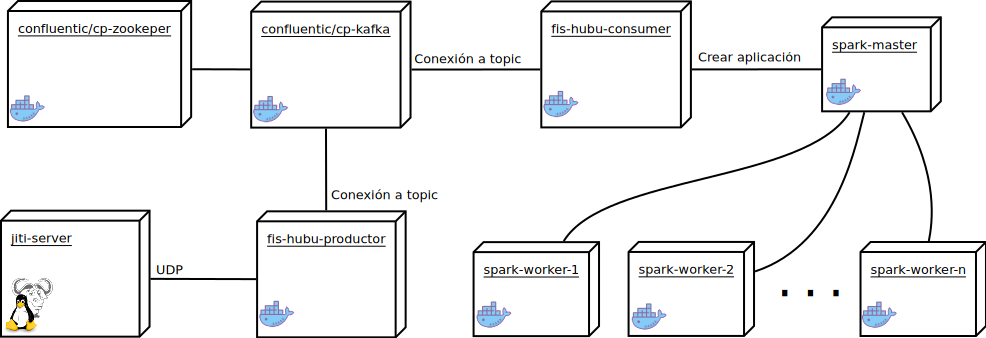
\includegraphics[width=\textwidth]{img/DespliegueDocker.png}
	\caption[Máquinas virtuales \textit{Docker} que implementan el flujo.]{Máquinas virtuales \textit{Docker} que implementan el flujo. Se muestra además la conexión con el servicio \textit{Jitsi} que recibe los datos y como se incorporan a \textit{fis-hubu-consumer}. Las máquinas \textit{fis-hubu-productor} y \textit{fis-hubu-consumer} son únicas para cada flujo, pero el resto son comunes a todos los flujos paralelos. La cantidad de \textit{workers} que se quisieran lanzar depende de la~\autoref{eq:fps}.}
	\label{fig:despligueDocker}
\end{figure}

Las máquinas \textit{fis-hubu} se han creado en exclusiva para este proyecto, funcionan sobre \textit{Ubuntu 18.04} y crean un entorno \textit{conda} para la correcta ejecución del algoritmo. Las modificaciones que fuesen necesarias para adaptar estas imágenes se encuentran en el anexo~\ref{sec:manualpro}. 

El orden de instancia de cada una de las máquinas es muy importante para que pueda ofrecerse el servicio adecuadamente. Lo primero que se ha de hacer es levantar las máquinas (en este orden) de \textit{Zookeeper}, \textit{Kafka}, nodo maestro de \textit{Spark} y por último los \textit{workers} que se deseen. Es importante asegurar el uso de una red virtual para que todos los \textit{dockers} se localicen entre sí o bien utilizar las conexiones con los puertos que se publiquen, aunque esta decisión no es la más acertada si el servidor puede ser usado con otros motivos.

Un detalle importante a tener en cuenta es que los nodos de \textit{Spark}, tanto el maestro como los esclavos deben tener acceso de alguna manera al código de ejecución, su entorno y sus características. Por tanto se hizo una modificación sobre estas imágenes para que heredasen de la imagen de \textit{fis-hubu-consumer} y así poder ejecutar cada nodo el código de \textit{Python} correctamente.

Una vez las máquinas <<servidoras>> estén disponibles, se pueden lanzar tanto \textit{fis-hubu-productor} como \textit{fis-hubu-consumer} garantizando un nombre identificativo para que no coincida con otros flujos que puedan aparecer.

Por último se han de inicializar el \textit{topic} de \textit{Kafka} en su máquina correspondiente, lanzar el \textit{script} de procesado en el \textit{fis-hubu-consumer} y el \textit{script} de encolado en el \textit{fis-hubu-productor}.

Para facilitar este proceso se han incorporado varios \textit{scripts} sobre \textit{bash} para automatizar la inicialización de las imágenes \textit{docker} y el lanzamiento de los \textit{scripts} de \textit{Python} necesarios.

El despliegue final se ha realizado utilizando una única máquina, pero el proceso sería similar si las imágenes \textit{docker} estuviesen lanzadas en un clúster de equipos.
  

\section{Extensibilidad}

Para que el flujo se pueda utilizar para el proceso que se quiera sobre los vídeos, se ha desarrollado una forma sencilla para que el programador pueda incrustar su código y se ejecute al final del flujo. Es importante que de utilizar algún objeto de ámbito global en esta extensión (como puede ser un modelo previamente cargado) es necesario que pueda ser serializable. En caso contrario, cuando \textit{Spark} desee enviar el objeto a un nodo esclavo, detendrá el flujo debido a no poder cargar el objeto.

A la hora de extender el algoritmo es importante conocer el tiempo de ejecución necesario para procesar un \textit{frame} y con ello elegir correctamente la cantidad de \textit{workers} de \textit{Spark} necesarios para que no se ralentice la ejecución global. Para elegir la cantidad de \textit{workers} necesarios, se utiliza la ecuación~\ref{eq:fps} que depende del tiempo de procesado medio, su desviación estándar y la tasa de \textit{fps} a procesar.

\begin{equation}\label{eq:fps}
\ceil{\frac{(t_{mean}+2t_{std})*\textrm{fps}}{1000}}
\end{equation}

\subsection{Análisis temporal del flujo}\label{sec:analisistemporal_flujo}

Si se quiere extender el flujo es importante primero conocer el tiempo que necesita de base para tenerlo en consideración a la hora de incorporar nuevas funcionalidades al flujo y aumentar el número de \textit{workers} para mantener el \textit{status} de tiempo real.

Para analizar el tiempo del flujo se creó una simulación del mismo que calculase el tiempo de procesado de cada uno de los fotogramas para posteriormente calcular la media y la desviación. Concretamente se utilizaron un total de $4863$ fotogramas analizados diez veces. Además se discriminó entre sin almacenar el fotograma y almacenándolo, y se estudiaron el flujo sin procesar (únicamente la deserialización) o con el pre-procesado completo (detección y anonimización del rostro y reparación del brillo y el contraste). Las medidas se calcularon sobre la ejecución de un procesador \textit{Intel Xeon} de 10 núcleos.

Pero antes de pasar a la muestra de los resultados es importante destacar que el uso de dos desviaciones típicas abarca la suficiente muestra de los datos como para considerarlo un dato adecuado. 

\begin{figure}
	\begin{subfigure}[b]{\textwidth}
		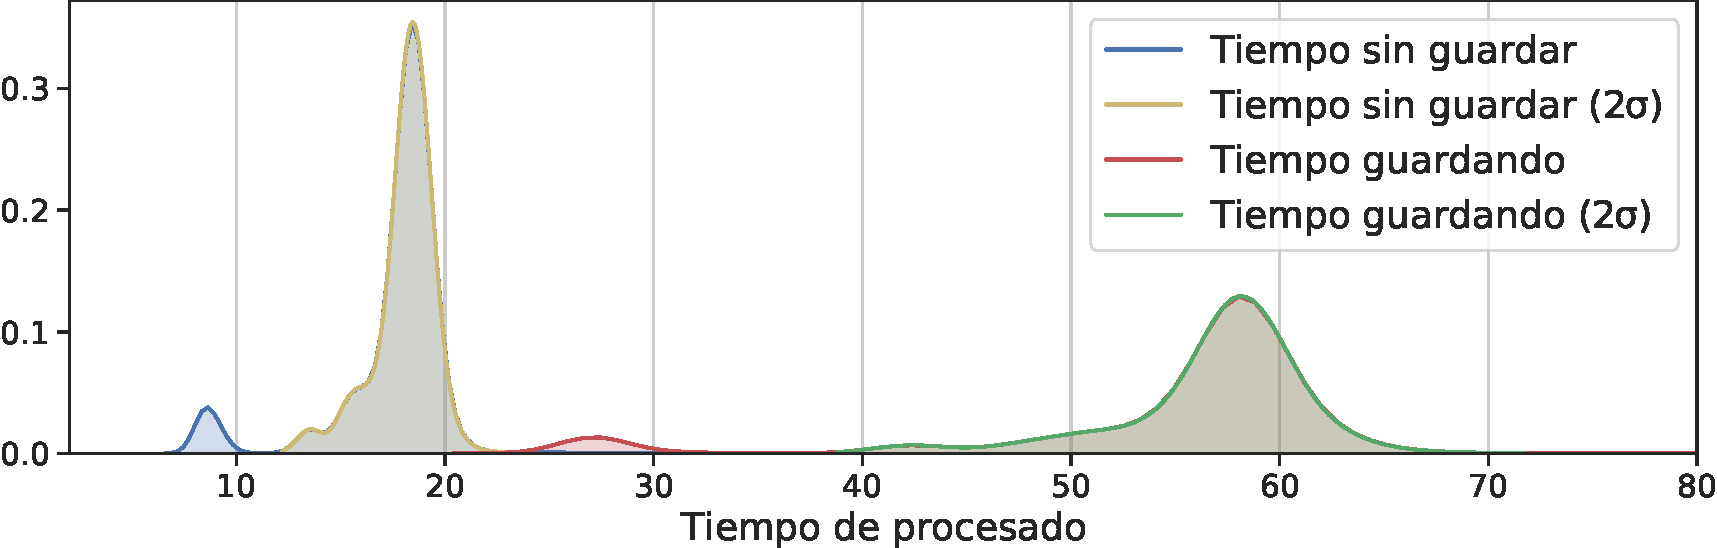
\includegraphics[width=\textwidth]{TiemposSinAccionDist.pdf}
		\caption{Imagen sin preprocesado.}
	\end{subfigure}
	\begin{subfigure}[b]{\textwidth}
		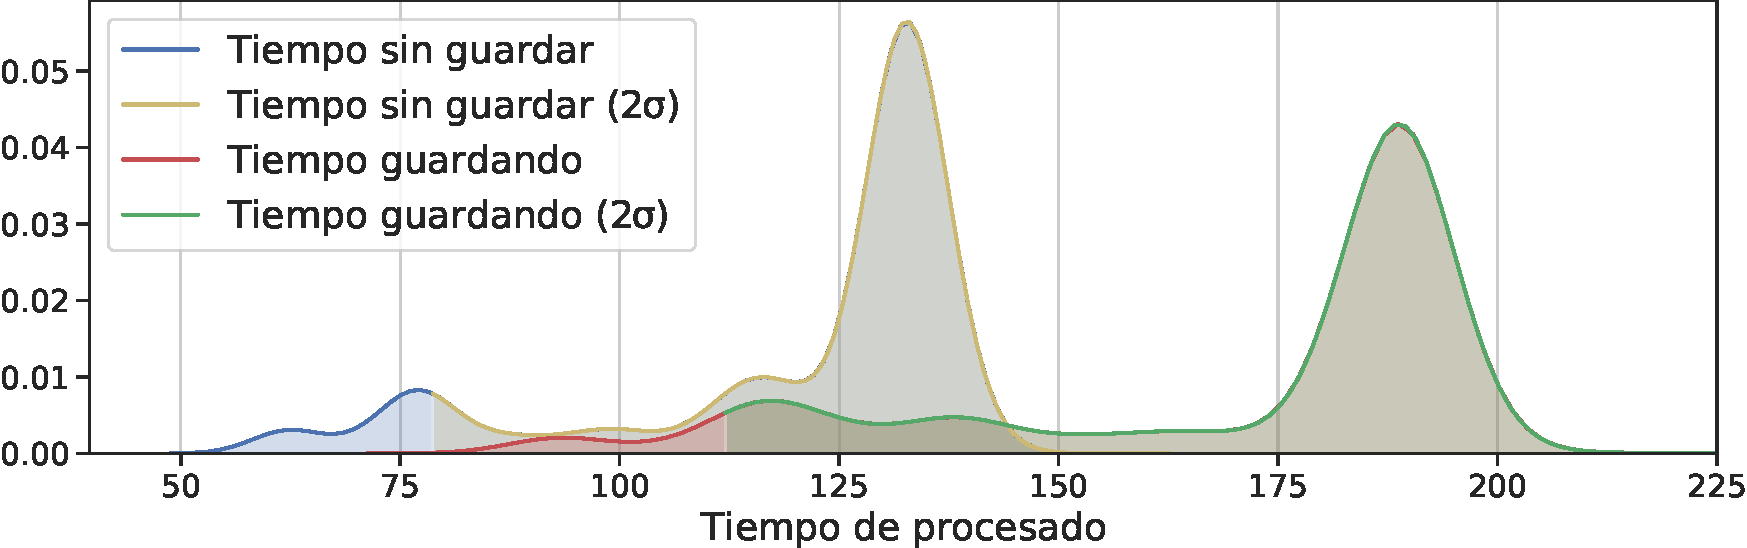
\includegraphics[width=\textwidth]{TiemposPrevioDist.pdf}
		\caption{Imagen con preprocesado.}
	\end{subfigure}
	\caption{Distribución de los datos temporales para el proceso del flujo sobre una imagen.}
	\label{fig:dist1}
\end{figure}


En la figura~\ref{fig:dist1} se pueden observar las distribuciones temporales para los casos considerados. La regla de las dos sigmas se cumple siempre con las distribuciones normales, sin embargo, aunque la distribución no es una normal si que asemeja su forma y abarca principalmente los datos temporales mayores por lo que se puede garantizar que el usar dos sigmas es suficiente rango temporal para el cálculo de \textit{workers}.

En la figura~\ref{fig:dist2} se observa la distribución estadística de los datos. Como es esperable el guardar las imágenes necesita de un tiempo considerablemente mayor. Los datos sin procesar la imagen son significativamente bajos, incluso la media sin guardar está en $17.5$ milisegundos, lo que alcanzaría un procesado de casi $60$ \textit{fps} para cada \textit{worker}. Son métricas muy buenas si se quiere extender el flujo que no necesiten la anonimización del rostro (como en cámaras de vigilizancia) o que ya vengan contrastadas. En el caso del preprocesado necesita de media $464$ milisegundos, que apenas da para procesar dos fotogramas por segundo.

\begin{figure}[h]
	\begin{subfigure}[b]{\textwidth}
		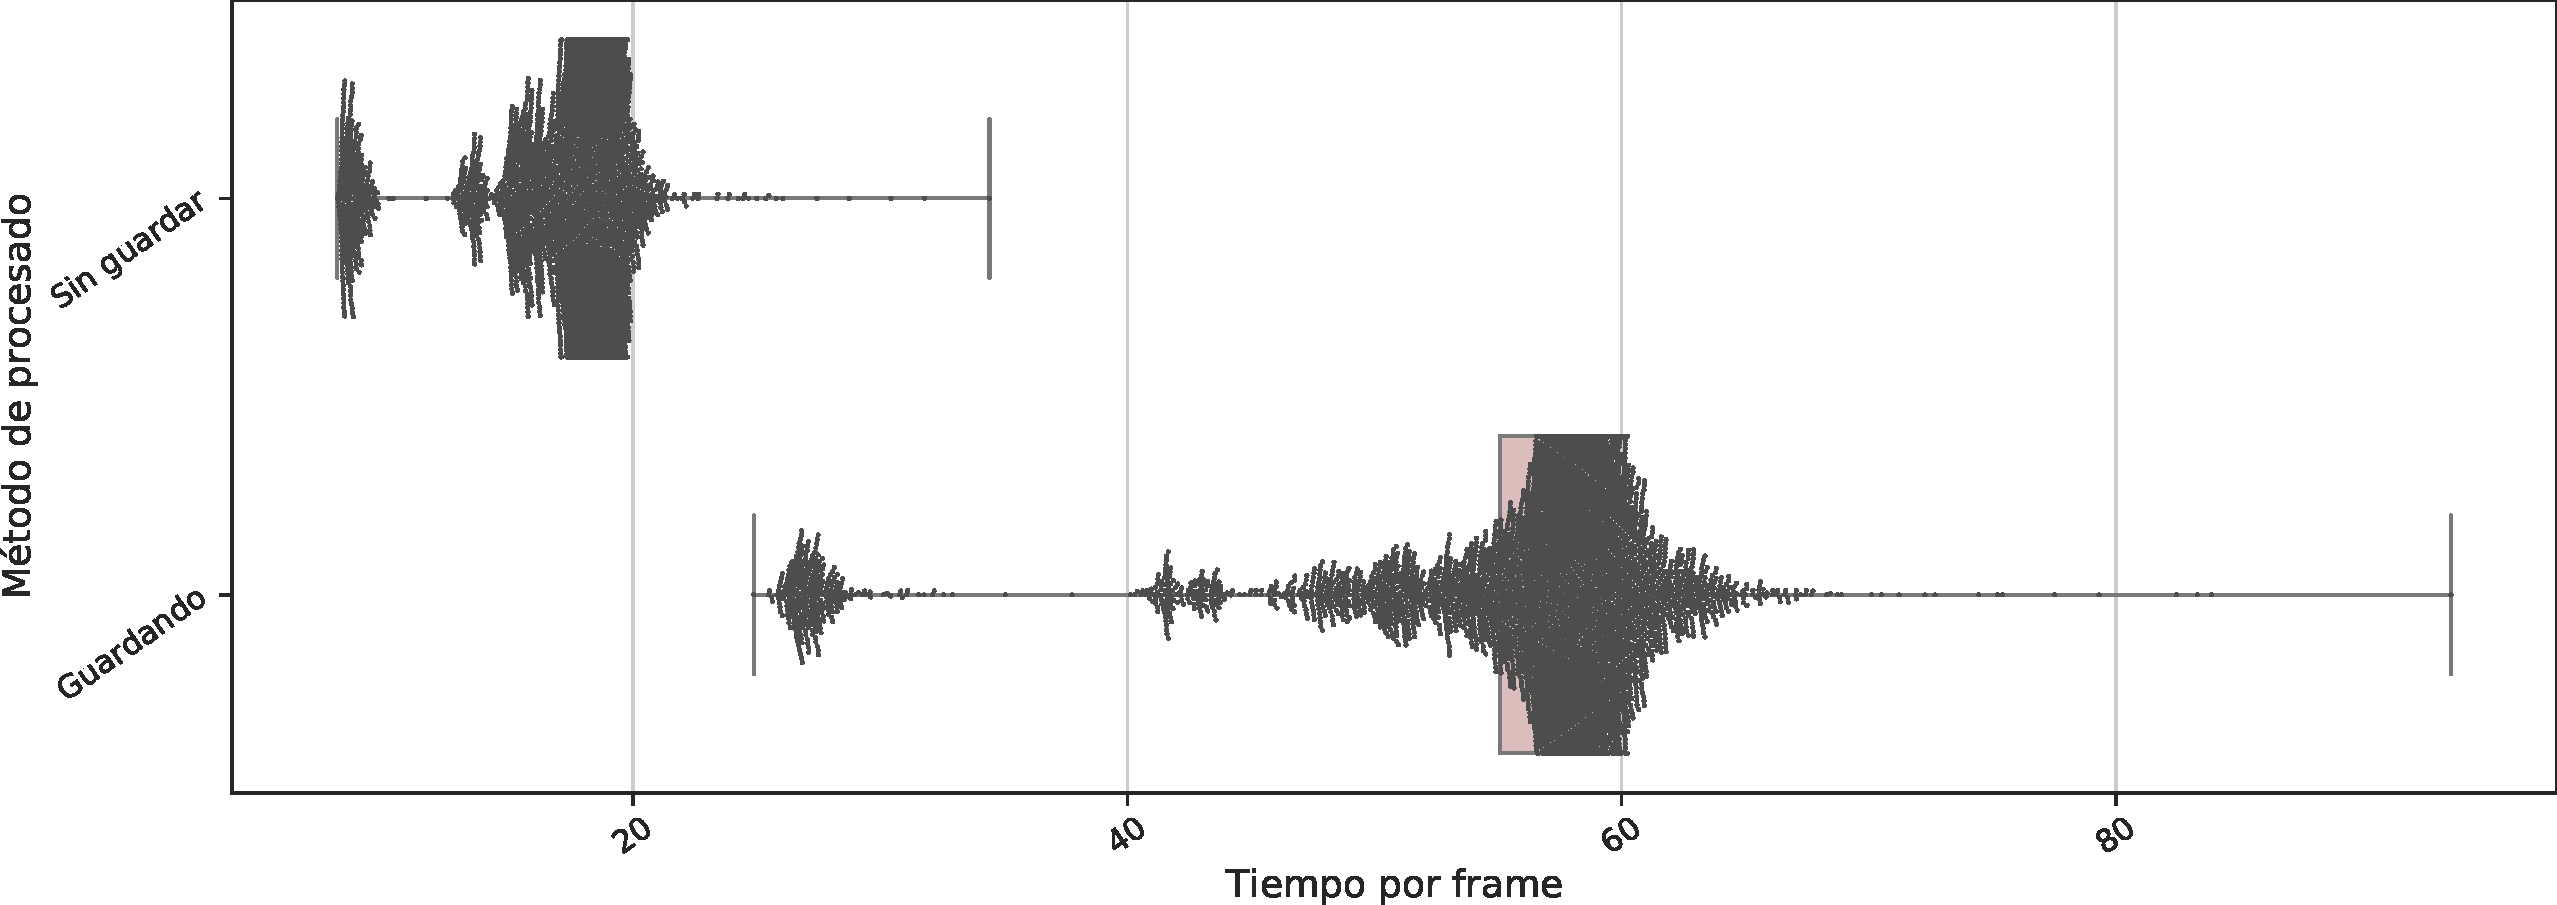
\includegraphics[width=\textwidth]{TiemposSinAccion.pdf}
		\caption{Imagen sin preprocesado.}
	\end{subfigure}
	\begin{subfigure}[b]{\textwidth}
		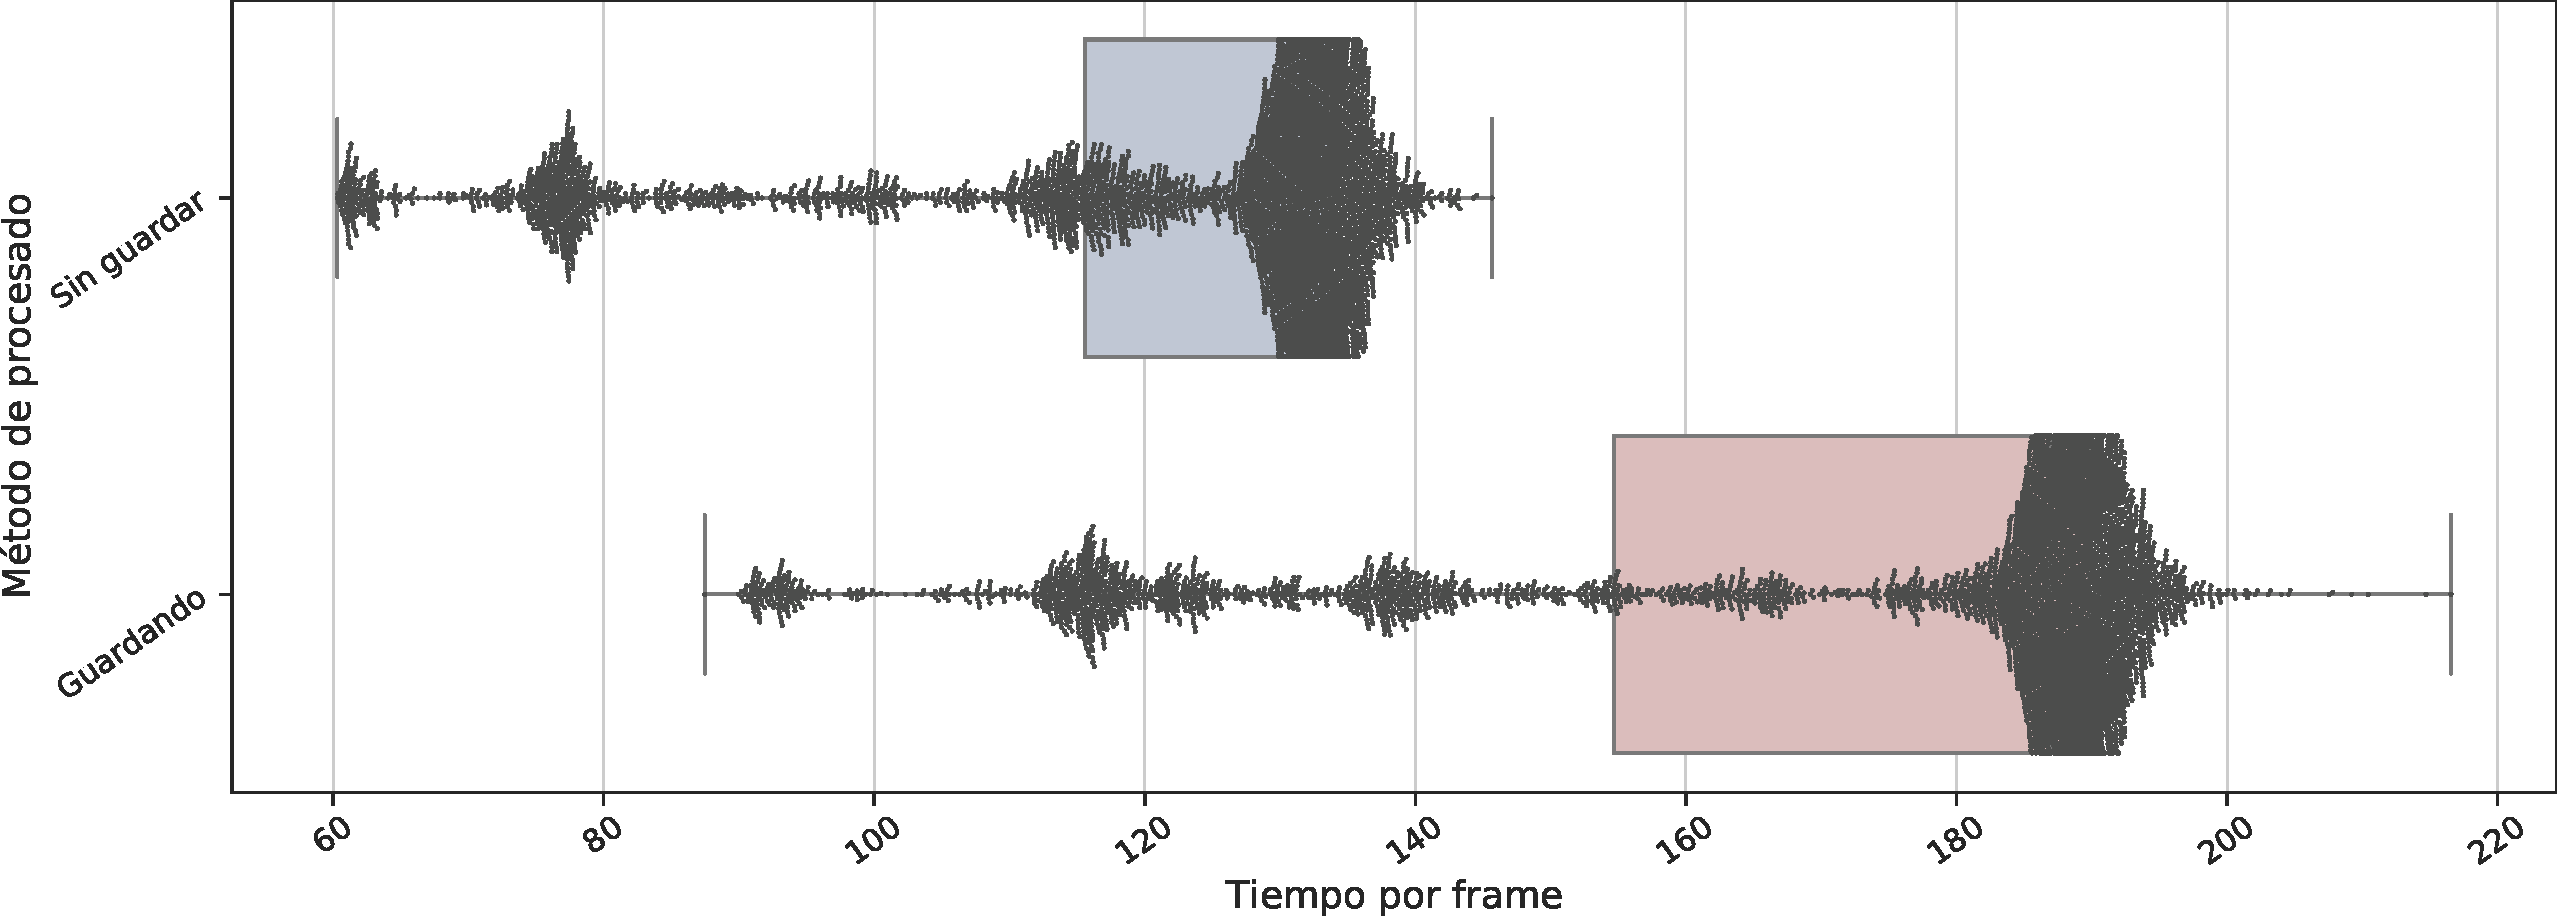
\includegraphics[width=\textwidth]{TiemposPrevio.pdf}
		\caption{Imagen con preprocesado.}
	\end{subfigure}
	\caption{Gráficos de bigotes con la distribución estadística de los datos temporales para el proceso del flujo sobre una imagen.}
	\label{fig:dist2}
\end{figure}

Con estos resultados, usando la \autoref{eq:fps}, podemos ver en la~\autoref{tab:workers1} la cantidad de \textit{workers} necesarios para ofrecer un procesado en tiempo real.

\begin{table}[h]
	\begin{center}
		\begin{tabular}{c  c c c c  }
			\toprule
			\multirow{2}{1.5cm}{\textbf{Tasa de \textit{fps}}}& \multicolumn{2}{c}{\textbf{Sin guardar}} & \multicolumn{2}{c}{\textbf{Guardando}}\\
			& \textbf{Sin procesar} & \textbf{Preprocesado} & \textbf{Sin procesar} & \textbf{Preprocesado}\\
			\otoprule
			\textbf{5 \textit{fps}} & 1 & 2 &1 & 3\\
			\textbf{15 \textit{fps}} & 1 & 1 &2 & 4\\
			\bottomrule
		\end{tabular}
	\end{center}
	\caption{N.º de \textit{workers} necesarios según el proceso a realizar.}
	\label{tab:workers1}
\end{table}


\subsection{Integración con el modelo de detección de esqueleto del paciente}

Se ha querido comprobar que la arquitectura de colas presentada en este trabajo funcionase correctamente en el proyecto que la engloba. Para ello se ha juntado con el modelo de clasificación para la detección del esqueleto y el cálculo de la diferencia entre dos estados.

Siguiendo las indicaciones\footnote{Ver \autoref{sec:manualpro}.} para hacer extensible el algoritmo, es decir, incorporar nuevas funcionalidades se ha incluido dentro del fichero \texttt{extraOpt.py} las importaciones de las clases creadas por José Miguel Ramírez Sanz, así como la instancia de la interfaz para acceder al modelo.

El primer detalle a tener en cuenta es que el modelo tenía que instanciarse en el ámbito global de la aplicación para que fuese serializado y enviado a todos los \textit{workers} de \textit{spark} ya que necesita para cargar entre 4 y 6 segundos, un tiempo excesivo que se sumaría al análisis de cada fotograma. Sin embargo, la inicialización del flujo necesita más tiempo por lo que es muy importante lanzarlo lo antes posible para cuando lleguen los primeros fotogramas esté completamente cargado.

Junto con la dificultad temporal surgió también una dificultar en memoria, concretamente la memoria de la tarjeta gráfica. Cada instancia cargada del modelo reservaba entre 512 y 768 MiB de VRAM por lo que según la cantidad de \textit{workers} se necesita una mayor cantidad de memoria en el sistema. En el caso personal, que se contaba con una \textit{Nvidia 750 Ti} de 2 GiB de memoria solamente se podían ejecutar un \textit{worker} junto con el \textit{master}, teniendo en cuenta la ecuación~\ref{eq:fps} implicaría que solamente se podían analizar $12$ en el caso de utilizar solamente el procesado básico y una tase de $3$ en el caso del flujo completo. Teniendo en cuenta las necesidades del tiempo real este dispositivo no es adecuado.

Al utilizar las GPU de la máquina \textit{gamma} del grupo \textit{ADMIRABLE}, que cuenta con tres \textit{Nvidia Titan Xp} de 12 GiB de memoria cada una se podían llegar a utilizar un total de 47 \textit{workers} junto con el nodo \textit{master}. Permitiendo así unas tasas de \textit{fps} de $288$ en el caso de solo usar el procesamiento básico y de $73$ con el flujo completo. Si los vídeos se mantienen con los \textit{15} fps se pueden tener $4$ flujos simultaneos y en el caso de reducir la tasa a 5 se pueden tener hasta $14$ flujos.


\subsection{Análisis temporal del flujo con toda la integración}\label{sec:analisistemporal}

Tal como se muestra en la \autoref{sec:analisistemporal_flujo} se realiza el mismo experimento con el flujo completo, es decir, se incorpora al preprocesado el modelo creado para este proyecto. En la \autoref{fig:boxplotTotal} se puede observar la distribución estadística de los datos evaluados. La media sin guardar la imagen es de $464$ ms y guardando de $626$ ms, las desviaciones típicas son de $86.5$ y $98.7$ respectivamente.

\begin{figure}[h]
	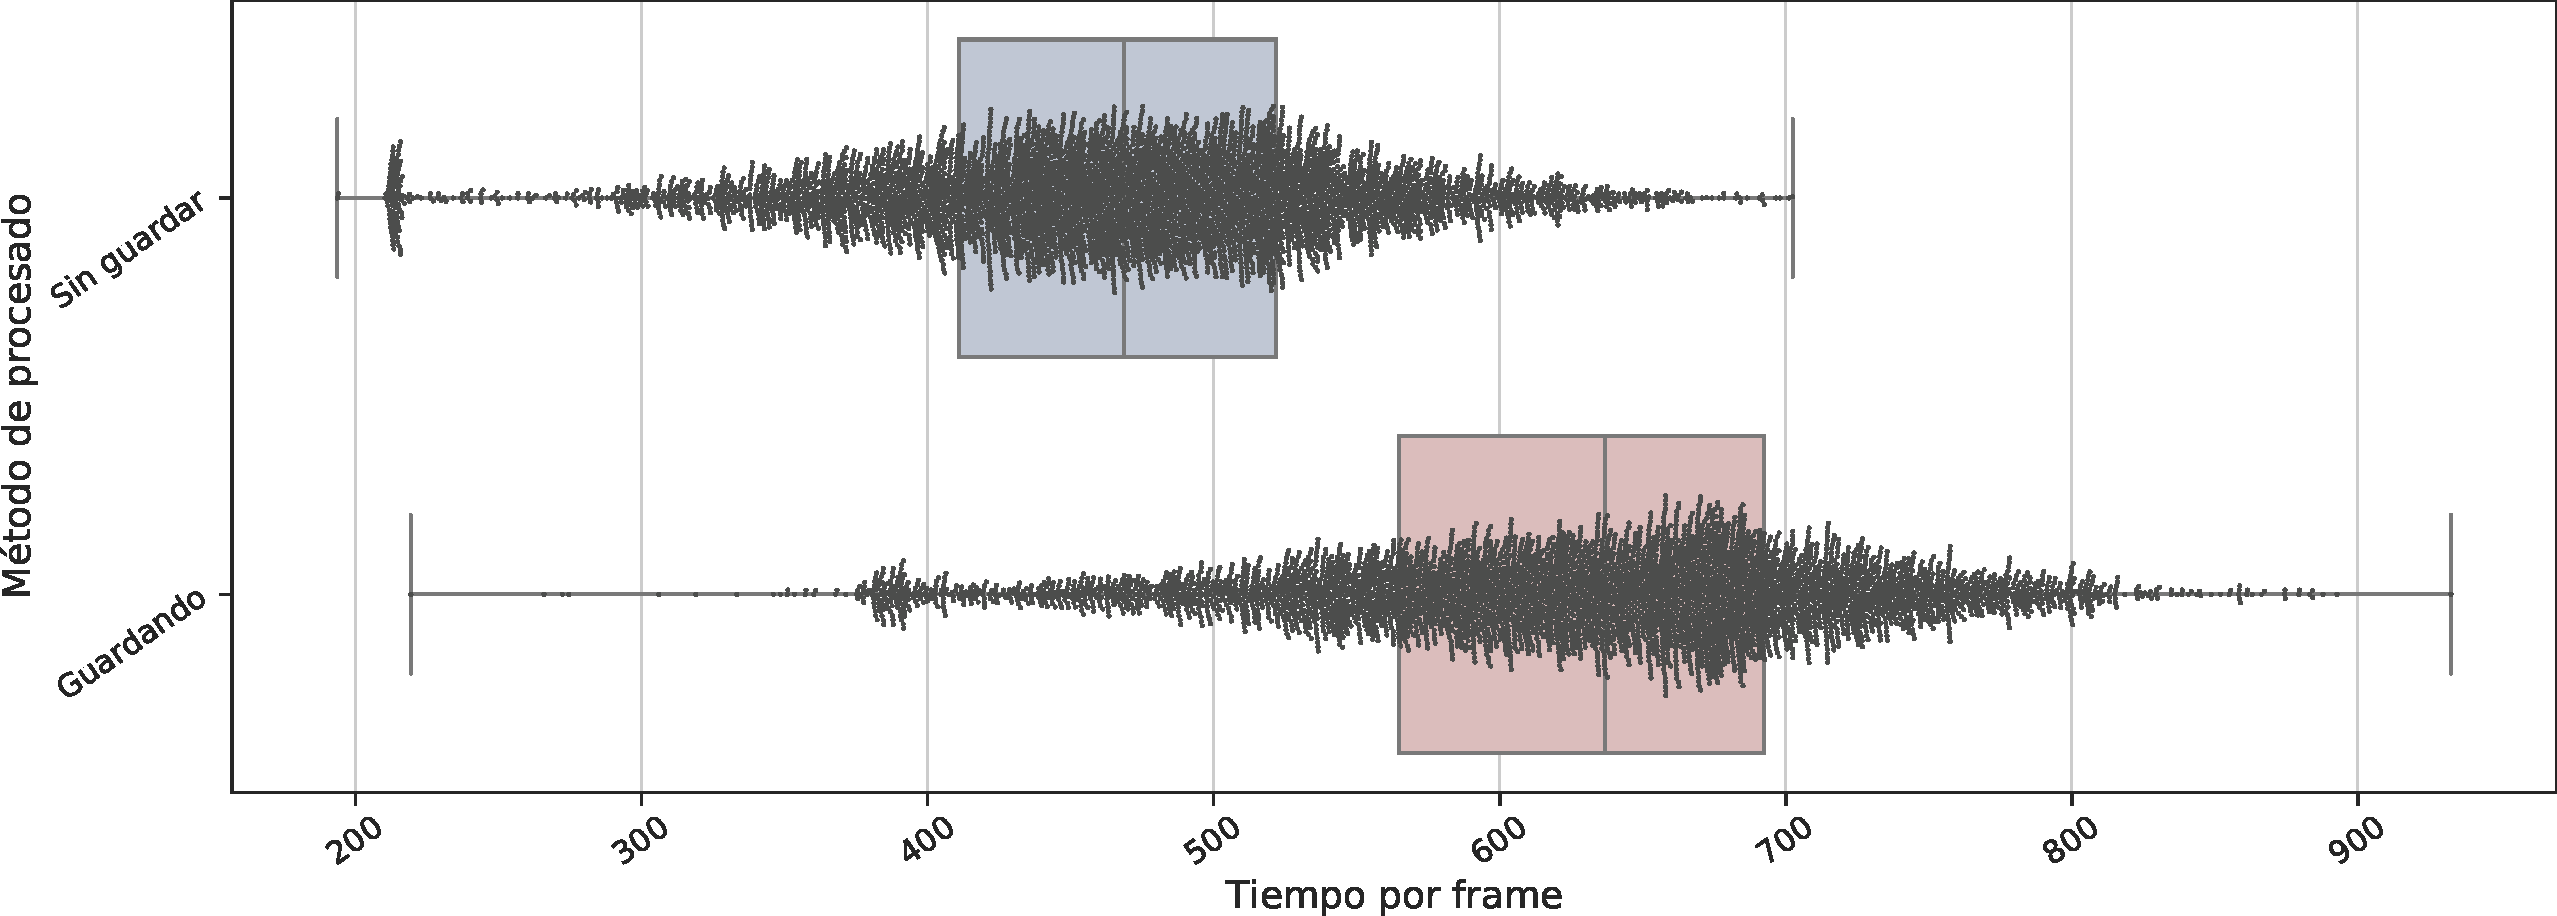
\includegraphics[width=\textwidth]{TiemposSumados.pdf}
	\caption{Gráficos de bigotes con la distribución estadística de los datos temporales para el proceso del flujo completo sobre una imagen.}
	\label{fig:boxplotTotal}
\end{figure}

Se necesitan, utilizando 15 \textit{fps} al menos 10 \textit{workers} si no se guarda y 13 en caso contrario. Por otro lado, de utilizar 5 \textit{fps} se necesitan 4 y 5 \textit{workers} sin guardar y guardando los fotogramas respectivamente.